% ---------------------------------------------------------------------------
% ---------------------------------------------------------------------------
% Modelo LaTex para preparação do documento final de Monografia TCC
% O modelo está em conformidade com ABNT NBR
% Faculdade do Piaui
% ---------------------------------------------------------------------------
% ---------------------------------------------------------------------------

\documentclass[
	% -- opções da classe memoir --
	12pt,					% tamanho da fonte
	openright,				% capítulos começam em pág ímpar (insere página vazia caso preciso)
	twoside,					% para impressão em verso e anverso. Oposto a oneside
	a4paper,					% tamanho do papel. 
	% -- opções da classe abntex2 --
	%chapter=TITLE,			% títulos de capítulos convertidos em letras maiúsculas
	%section=TITLE,			% títulos de seções convertidos em letras maiúsculas
	%subsection=TITLE,		% títulos de subseções convertidos em letras maiúsculas
	%subsubsection=TITLE,	% títulos de subsubseções convertidos em letras maiúsculas
	% -- opções do pacote babel --
	english,					% idioma adicional para hifenização
	%french,					% idioma adicional para hifenização
	%spanish,				% idioma adicional para hifenização
	brazil					% o último idioma é o principal do documento
	]{abntex2}

% ---------------------
% Pacotes OBRIGATÓRIOS
% ---------------------
\usepackage{lmodern}				% Usa a fonte Latin Modern			
\usepackage[T1]{fontenc}			% Selecao de codigos de fonte.
\usepackage[utf8]{inputenc}		% Codificacao do documento (conversão automática dos acentos)
\usepackage{lastpage}			% Usado pela Ficha catalográfica
\usepackage{indentfirst}			% Indenta o primeiro parágrafo de cada seção.
\usepackage{color}				% Controle das cores
\usepackage{graphicx,graphicx}	% Inclusão de gráficos
\usepackage{epsfig,subfig}		% Inclusão de figuras
\usepackage{microtype} 			% Melhorias de justificação
\graphicspath{{figs/}}

% ---------------------
		
% ---------------------
% Pacotes ADICIONAIS
% ---------------------
\usepackage{pdfpages}


\usepackage{lipsum}						% Geração de dummy text
\usepackage{amsmath,amssymb,mathrsfs}	% Comandos matemáticos avançados 
\usepackage{setspace}  					% Para permitir espaçamento simples, 1 1/2 e duplo
\usepackage{verbatim}					% Para poder usar o ambiente "comment"
\usepackage{tabularx} 					% Para poder ter tabelas com colunas de largura auto-ajustável
\usepackage{afterpage} 					% Para executar um comando depois do fim da página corrente
\usepackage{url} 						% Para formatar URLs (endereços da Web)

%\usepackage[style=long,nonumberlist,toc,xindy,nomain]{glossaries}
				% para fazer glossario	
\usepackage{glossaries}	
\loadglsentries{extras/glossary}
\makeglossaries

%% para referenciar abreviaturas
\makeatletter
\def\namedlabel#1#2{\begingroup
	#2%
	\def\@currentlabel{#2}%
	\phantomsection\label{#1}\endgroup
}
% ---------------------

% ---------------------
% Pacotes de CITAÇÕES
% ---------------------
\usepackage[brazilian,hyperpageref]{backref}	% Paginas com as citações na bibl
\usepackage[alf]{abntex2cite}				% Citações padrão ABNT (alfa)
%\usepackage[num]{abntex2cite}				% Citações padrão ABNT (numericas)
% ---------------------

\usepackage{ulem}

\definecolor{mypurple}{rgb}{0.8,0.5,1}
\newcommand{\fulano}[1]{\textcolor{mypurple}{#1}}

\newcommand{\source}[1]{\caption*{Fonte: {#1}} }

% Configurações de CITAÇÕES para abntex2
% --- 
% CONFIGURAÇÕES DE PACOTES
% --- 

% ---
% Configurações do pacote backref
% Usado sem a opção hyperpageref de backref
\renewcommand{\backrefpagesname}{Citado na(s) página(s):~}
% Texto padrão antes do número das páginas
\renewcommand{\backref}{}
% Define os textos da citação
\renewcommand*{\backrefalt}[4]{
	\ifcase #1 %
		Nenhuma citação no texto.%
	\or
		Citado na página #2.%
	\else
		Citado #1 vezes nas páginas #2.%
	\fi}%
% ---

% Inclusão de dados para CAPA e FOLHA DE ROSTO (título, autor, orientador, etc.)
% ---
% Informações de dados para CAPA e FOLHA DE ROSTO
% ---
\titulo{Desenvolvimento de subsistemas para rotina de inspeção do Robô ELIR}
\autor{Carlos Pereira\\
	Cleber Couto Filho\\
	Davi Costa\\	
	Ícaro Queiroz\\}
\local{Salvador-BA}
\data{\today}
\orientador{Professor MSc. Marco Reis}
\coorientador{Professor(a) Titulação  Coorientador}
\instituicao{%
  Centro Universitário SENAI CIMATEC}
\tipotrabalho{Trabalho de Conclusão de Curso (TCC)}
% O preambulo deve conter o tipo do trabalho, o objetivo,
% o nome da instituição e a área de concentração
\preambulo{\textbf{Trabalho de Conclusão de Curso} apresentado ao Centro Universitário SENAI CIMATEC como requisito parcial para a obtenção do grau de Bacharel em Engenharia Elétrica.}
% ---

% Inclui Configurações de aparência do PDF Final
%  Configurações de aparência do PDF final
% NÃO ALTERAR!!!

% alterando o aspecto da cor azul
\definecolor{blue}{RGB}{41,5,195}

% informações do PDF
\makeatletter
\hypersetup{
     	%pagebackref=true,
		pdftitle={\@title}, 
		pdfauthor={\@author},
    		pdfsubject={\imprimirpreambulo},
	    pdfcreator={LaTeX with abnTeX2},
		pdfkeywords={abnt}{latex}{abntex}{abntex2}{trabalho acadêmico}, 
		colorlinks=true,       		% false: boxed links; true: colored links
    		linkcolor=blue,          	% color of internal links
    		citecolor=blue,        		% color of links to bibliography
    		filecolor=magenta,      		% color of file links
		urlcolor=blue,
		bookmarksdepth=4
} 
\makeatother
% --- 

% O tamanho da identação do parágrafo é dado por:
\setlength{\parindent}{1.3cm}

% Controle do espaçamento entre um parágrafo e outro:
\setlength{\parskip}{0.2cm}  % tente também \onelineskip

% ---------------------
% Compila o indice
% ---------------------
\makeindex
% ---------------------



%%%%%%%%%%%%%%%%%%%%%%%%%%%
%%  INICIO DO DOCUMENTO  %%
%%%%%%%%%%%%%%%%%%%%%%%%%%%
\begin{document}

% Retira espaço extra obsoleto entre as frases.
\frenchspacing

% ----------------------------------------------------------
% ELEMENTOS PRÉ-TEXTUAIS (Capa, Resumo, Abstract, etc.)
% ----------------------------------------------------------
\pretextual

% Capa
% ---
% Impressão da Capa
% ---
  \begin{capa}%
    \begin{figure}[h!]%
        \centering%
        
\includegraphics[scale=0.4]{figs/logo_senai.jpeg}%
      \end{figure}%
    \center
	\ABNTEXchapterfont\large{Centro Universitário SENAI CIMATEC\\Curso de Bacharelado em Engenharia Elétrica}
	%\vspace{1.5cm}

    \vfill
    \ABNTEXchapterfont\bfseries\LARGE\imprimirtitulo
    \vfill

	%\vfill
	\ABNTEXchapterfont\large\imprimirautor
	\vfill
%
    \large\imprimirlocal, \large\imprimirdata

    \vspace*{1cm}
  \end{capa}
% ---

% Folha de rosto (o * indica que haverá a ficha bibliográfica)
\imprimirfolhaderosto*

% Resumo e Abstract
% ---
% RESUMOS
% ---

% RESUMO em português
\setlength{\absparsep}{18pt} % ajusta o espaçamento dos parágrafos do resumo
\begin{resumo}
 Segundo a ABNT, o resumo deve ressaltar o
 objetivo, o método, os resultados e as conclusões do documento. A ordem e a extensão
 destes itens dependem do tipo de resumo (informativo ou indicativo) e do
 tratamento que cada item recebe no documento original. O resumo deve ser
 precedido da referência do documento, com exceção do resumo inserido no
 próprio documento. (\ldots) As palavras-chave devem figurar logo abaixo do
 resumo, antecedidas da expressão Palavras-chave:, separadas entre si por
 ponto e finalizadas também por ponto.

 \textbf{Palavras-chaves}: latex. abntex. editoração de texto.
\end{resumo}

% ABSTRACT in english
\begin{resumo}[Abstract]
 \begin{otherlanguage*}{english}
   This is the english abstract.

   \vspace{\onelineskip}
 
   \noindent 
   \textbf{Keywords}: latex. abntex. text editoration.
 \end{otherlanguage*}
\end{resumo}

% Lista de ilustrações
\pdfbookmark[0]{\listfigurename}{lof}
\listoffigures*
\cleardoublepage

% Lista de tabelas
\pdfbookmark[0]{\listtablename}{lot}
\listoftables*
\cleardoublepage

% Lista de abreviaturas e siglas
\begin{siglas}
  \item[ABNT] Associação Brasileira de Normas Técnicas
  \item[abnTeX] ABsurdas Normas para TeX
  \item [\namedlabel{itm:ros}{ROS}] \textit{Robot Operating System}
  \item [\namedlabel{itm:urdf}{URDF}] \textit{Unified Robot Description Format}
  \item [\namedlabel{itm:elir}{ELIR}] \textit{Electrial Line Inspection Robot}
\end{siglas}

% Lista de símbolos
\begin{simbolos}
  \item[$ \Gamma $] Letra grega Gama
  \item[$ \Lambda $] Lambda
  \item[$ \zeta $] Letra grega minúscula zeta
  \item[$ \in $] Pertence
\end{simbolos}

% Inserir o SUMÁRIO
\pdfbookmark[0]{\contentsname}{toc}
\tableofcontents*
\cleardoublepage

% ----------------------------------------------------------
% ELEMENTOS TEXTUAIS (Capítulos)
% ----------------------------------------------------------
\textual
% Elementos textuais com numeração arábica
\pagenumbering{arabic}
% Reinicia a contagem do número de páginas
\setcounter{page}{1}

% Inclui cada capitulo da Dissertação
% ----------------------------------------------------------
% Introdução 
% Capítulo sem numeração, mas presente no Sumário
% ----------------------------------------------------------

\chapter*[Introdução]{Introdução}
\addcontentsline{toc}{chapter}{Introdução}

Este documento segue as normas estabelecidas pela~\citeonline[3.1-3.2]{NBR6028:2003}. \lipsum[30-34]

\section*{Motivação}\label{sec:motivacao}
\addcontentsline{toc}{section}{Motivação}

\lipsum[35]

\section*{Objetivos}\label{sec:objetivos}
\addcontentsline{toc}{section}{Objetivos}

Como objetivo geral este trabalho propõe...

Para isso, objetivos específicos foram assim definidos:

\begin{itemize}
\item especificar objetivos específicos
\item listar objetivos específicos
\end{itemize}

\section*{Organização do documento}\label{sec:objetivos}
\addcontentsline{toc}{section}{Organização do documento}

Parte I, Parte II, Parte III... \lipsum[32]


% PARTE - Define a divisão do documento em partes (Não é obrigatório)
%\part{Preparação da pesquisa}
%\begin{center}
	\Large \textbf{Referências}
\end{center}
	
	[1] TUDE, Eduardo. Enlace rádio digital ponto a ponto. 2004.

\chapter{Concept And Design}\label{cap:CnptDsng}

\section{Arquitetura Geral}\label{sec:arqgrl}
\lipsum[5]
\begin{figure}[h]
	\centering
	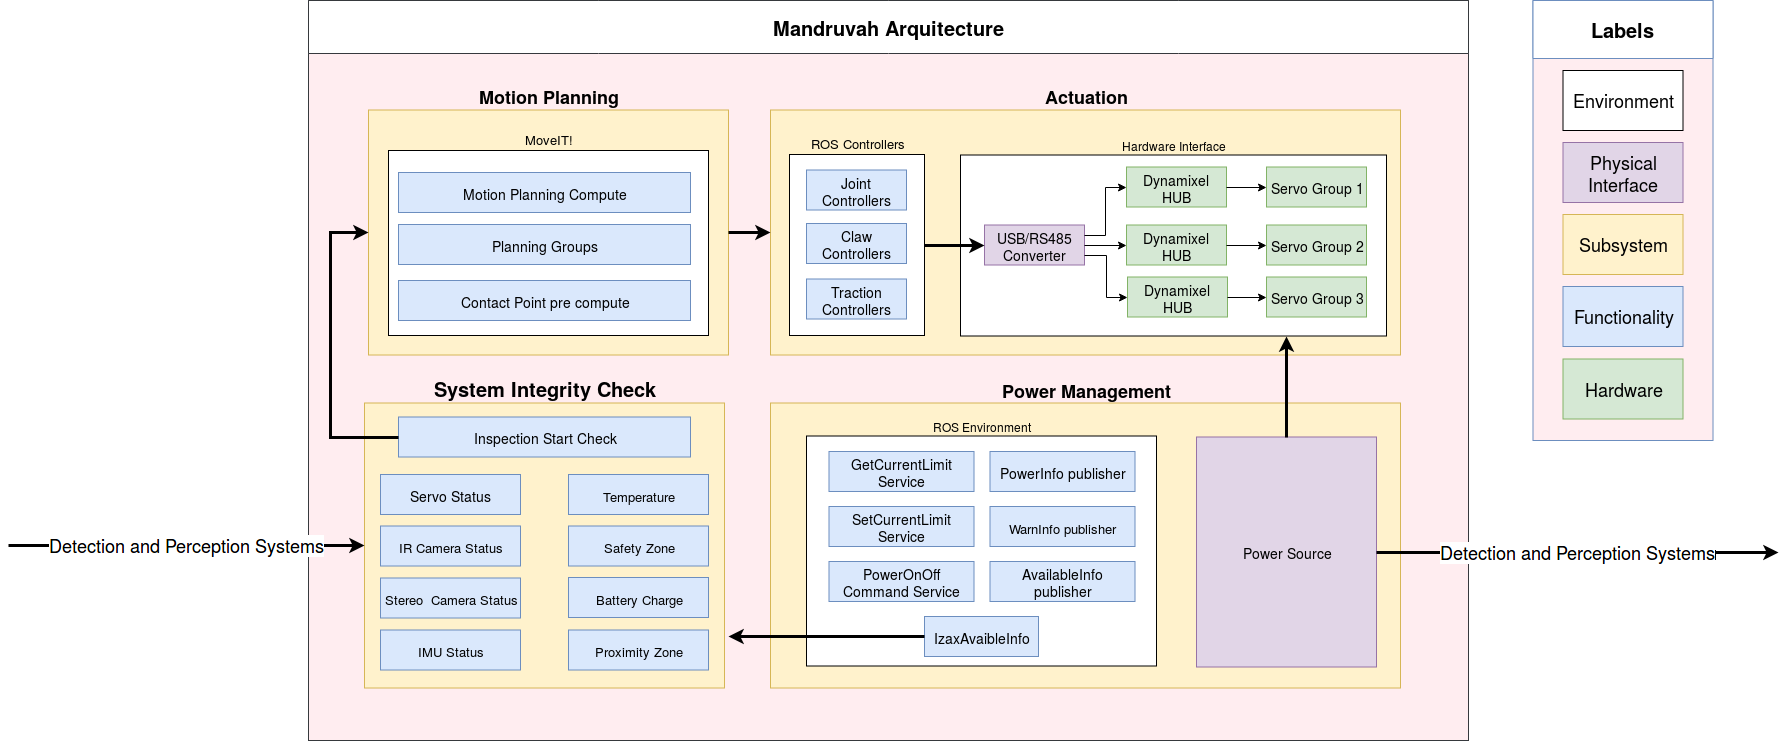
\includegraphics[width=1\textwidth]{Arquitetura.png}
	\caption{Arquitetura Geral do sistema de movimentação}
	\label{fig:arq_geral}
	\source{Própria}
\end{figure} 
\lipsum[5]


\section{Especificação Funcional}
\lipsum[3]

\subsection{Motion Planning}
\subsubsection{Definição da funcionalidade}
\lipsum[3]
\subsubsection{Dependências}
\lipsum[5]

\subsubsection{Premissas Necessárias}
\lipsum[1]
\begin{itemize}
	\item \lipsum[1]
	\item \lipsum[1]
	\item \lipsum[1]
\end{itemize}
\subsubsection{Descrição da Funcionalidade}
\lipsum[5]

\begin{figure}[h]
	\centering
	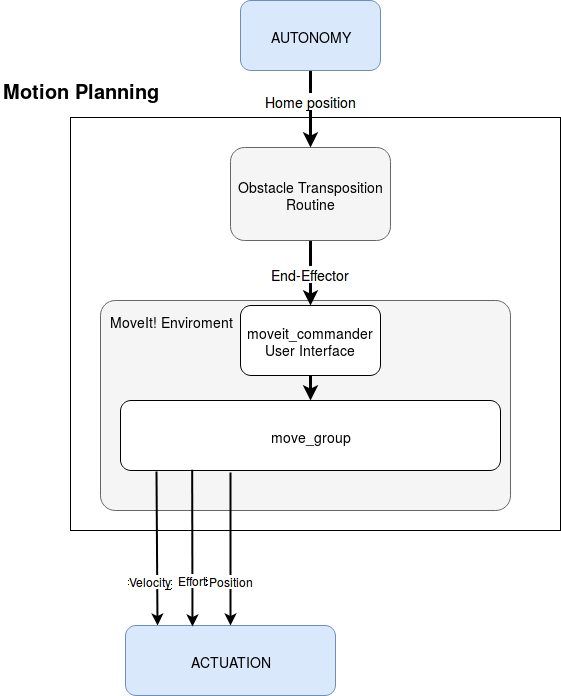
\includegraphics[width=0.6\textwidth]{motion_plan_func.png}
	\caption{Fluxograma de funcionamento da funcionalidade de Motion Planning}
	\label{fig:flux_motion}
	\source{Própria}
\end{figure}

\subsubsection{Saídas}
Por meio da compatibilização do \gls{moveit} com o \ref{itm:ros}, a saída dessa funcionalidade são os comandos de velocidade, esforço e posição para cada junta do robô.
\subsection{Actuation}
\subsubsection{Definição da funcionalidade}
\lipsum[2]
\subsubsection{Dependências}
\lipsum[5]

\subsubsection{Premissas Necessárias}
Para o correto funcionamento desse módulo, devem ser consideradas as seguintes premissas:
\begin{itemize}
	\item \lipsum[1]
	\item \lipsum[1]
	\item \lipsum[1]
\end{itemize}
\subsubsection{Descrição da Funcionalidade}
\lipsum[5]
	\begin{figure}[h]
		\centering
		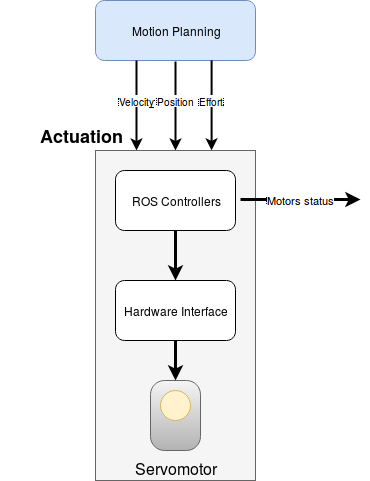
\includegraphics[width=0.6\textwidth]{actuation_depen.png}
		\caption{Fluxograma da funcionalidade Actuation}
		\label{fig:depen_actuation}
		\source{Própria}
	\end{figure}
\subsubsection{Saídas}
\lipsum[2]














% PARTE
%\part{Proposta}
\chapter{Proposta do trabalho}\label{cap:proposta}

Esse trabalho propõe... 

Mostrar o produto da pesquisa.

\section{Funcionamento}

\lipsum[67-73]

\section{Considerações Finais}

\lipsum[68]


% PARTE
%\part{Parte Final}
\chapter{Resultados e Discussão}\label{cap:resultados}

\lipsum[75]

\section{Apresentação dos dados coletados}

\lipsum[76-77]

\section{Análise dos dados}

\lipsum[78-80]

\section{Vantagens}

\lipsum[60-62]

\section{Limitações}

\lipsum[63-64]

\section{Considerações Finais}

\lipsum[31]
\chapter{Conclusão e Trabalhos Futuros}\label{cap:conclusao}

\lipsum[82-84]

\section{Trabalhos Futuros}

\lipsum[85] 

% ----------------------------------------------------------
% ELEMENTOS PÓS-TEXTUAIS (Referências, Glossário, Apêndices)
% ----------------------------------------------------------
\postextual

% Referências bibliográficas
\bibliography{bibliografia}

\printglossaries

% Glossário (Consulte o manual)
%\include{dados/}

% Apêndices
% ----------------------------------------------------------
% Apêndices
% ----------------------------------------------------------

% ---
% Inicia os apêndices
% ---
\begin{apendicesenv}

% Imprime uma página indicando o início dos apêndices
\partapendices

% ----------------------------------------------------------
\chapter{Título do primeiro apêncice}
% ----------------------------------------------------------

\lipsum[50] % Texto qualquer. REMOVER!!

% ----------------------------------------------------------
\chapter{Título do segundo apêndice}
% ----------------------------------------------------------
\lipsum[51-53] % Texto qualquer. REMOVER!!

\end{apendicesenv}
% ---

% Anexos
% ----------------------------------------------------------
% Apêndices
% ----------------------------------------------------------

% ---
% Inicia os anexos
% ---
\begin{anexosenv}

% Imprime uma página indicando o início dos anexos
\partanexos

% ---
\chapter{Nome do primeiro anexo}
% ---
\lipsum[30] % Texto qualquer. REMOVER!!

% ---
\chapter{Nome de outro anexo}
% ---

\lipsum[32] % Texto qualquer. REMOVER!!

\end{anexosenv}



% Índice remissivo (Consultar manual)
%\phantompart
%\printindex



\end{document}
